\subsection{Исследование свободных процессов в цепи второго порядка}

\begin{figure}[!h]
    \centering
    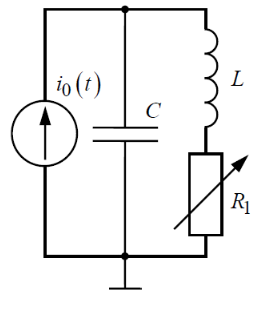
\includegraphics[width=4cm]{scheme_second_order.png}
    \caption{Схема для исследования}
    \label{fig:scheme_second_order}
\end{figure}

Соберём схему, изображённую на рис. \ref*{fig:scheme_second_order}.

\subsubsection{Расчеты по осциллограмме}

Снимем осциллограммы напряжения на резисторе в цепи
(рис. \ref*{fig:oscillograph_second_order}) при $R_1 = 0.5$ кОм (колебательный режим).

\begin{figure}[!h]
    \centering
    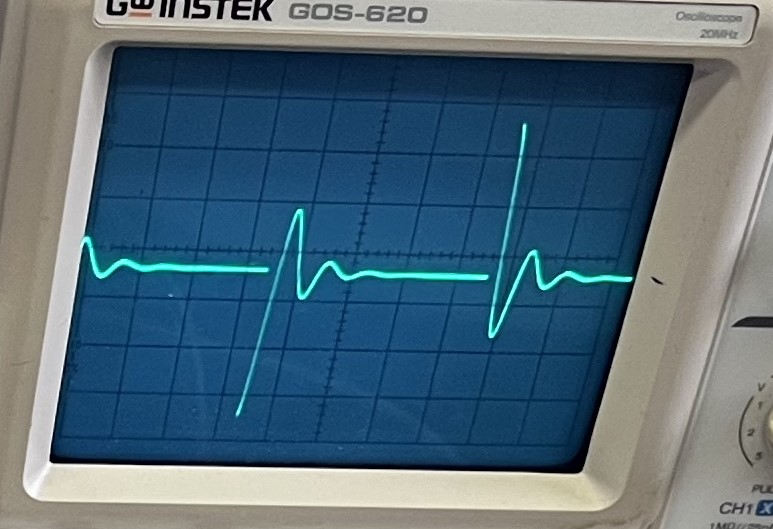
\includegraphics[width=0.8\textwidth]{oscillograph_second_order_vibr_IMG_7890.JPG}
    \caption{Осциллограмма напряжения в цепи второго порядка (колебательный режим)}
    \label{fig:oscillograph_second_order}
\end{figure}

По осциллограмме напряжения на конденсаторе получим значения собственной частоты:

\begin{figure}[!h]
    \centering
    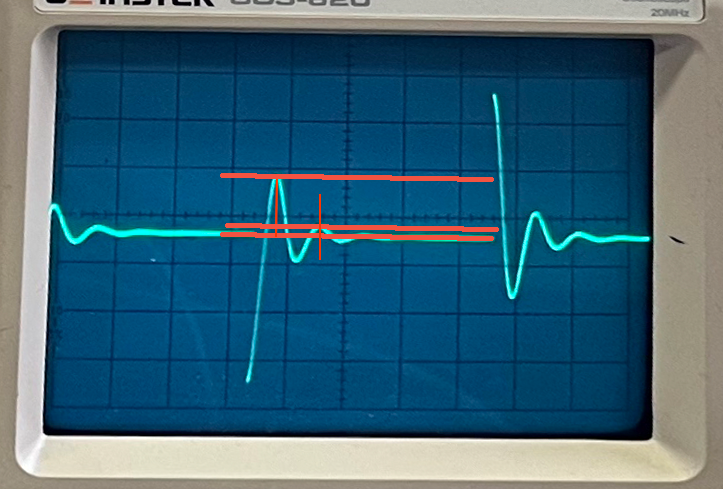
\includegraphics[width=0.6\textwidth]{ебейшие вычисления 2_IMG_7890.png}
    \caption{Осциллограмма напряжения на конденсаторе}
    \label{fig:culculations_second_order}
\end{figure}

Из рис. \ref*{fig:culculations_second_order} видно, что $U_1 = 0.24$ В, $U_2 = 0.06$ В, $T = 0.10$ мс.

Тогда коэффициент затухания равен

\[
    \alpha = \frac{\ln {(U_1 / U_2)} }{T}
    = \frac{\ln{(0.24/0.06)}}{0.10 \cdot 10^{-3}} \approx 14\ \text{кГц}
\]

Тогда собственные частоты равны

\[
    p_{1,2} = -\alpha \pm j \omega
    =  -\alpha \pm j \frac{2\pi}{T}
    = - 14 \pm j \frac{2\pi}{0.10 \cdot 10^{-3}} \approx -14 \pm 63j\ \text{кГц}
\]

Из рис. \ref*{fig:oscillograph_second_order_const} видно, что при $R_1 = 0$ колебания
практически не затухающие.

\begin{figure}[!h]
    \centering
    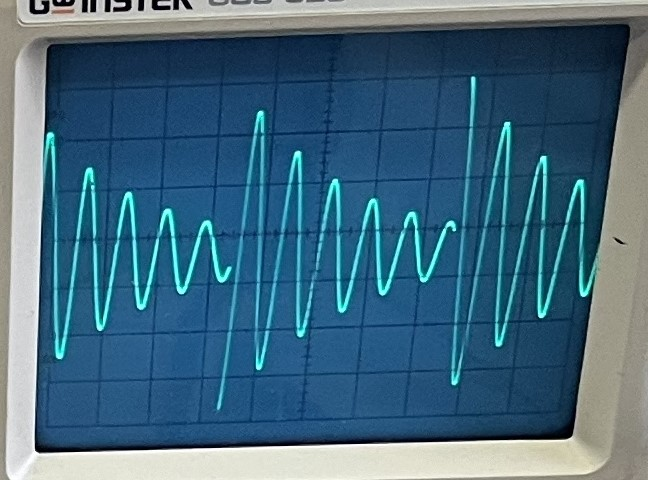
\includegraphics[width=0.8\textwidth]{oscillograph_second_order_const_vibr_IMG_7893.JPG}
    \caption{Осциллограмма напряжения в цепи второго порядка (незатухающие колебания)}
    \label{fig:oscillograph_second_order_const}
\end{figure}

Найдем период
колебаний $T = 0.08$ мс, тогда частота незатухающий
колебательный равна
\[
    \omega_0 = \frac{2\pi}{T}
    = \frac{2\pi}{0.08 \cdot 10^{-3}} \approx 78 \cdot 10^3\ \text{рад/с}
\]

Найдем добротность

\[
    Q = \\frac{\omega_0}{2\alpha}
    = \frac{78}{2 \cdot 14} \approx 2.78
\]

По осциллограмме напряжения получим значение постоянной времени
$\tau = 0.05$ мс при апериодическом режиме
(см. рис. \ref*{fig:culculations_second_order_aperiodic}).
Найдем собственную частоту цепи $p_1 = -\frac{1}{\tau} = -\frac{1}{0.05 \cdot 10^-3} \approx - 20$ кГц.

\begin{figure}[!h]
    \centering
    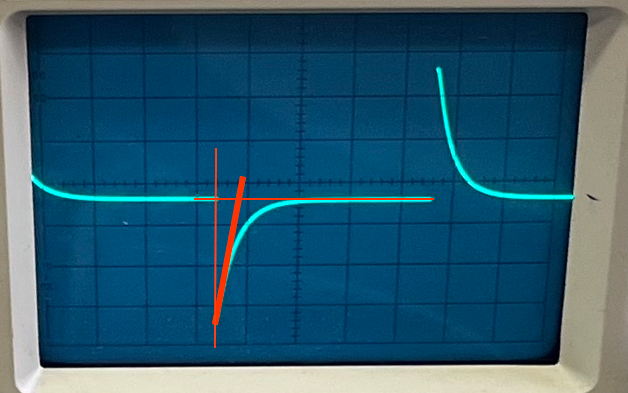
\includegraphics[width=0.6\textwidth]{ебейшие вычисления_3.png}
    \caption{Осциллограмма напряжения на конденсаторе}
    \label{fig:culculations_second_order_aperiodic}
\end{figure}

\subsubsection{Теоретические расчеты}

Найдем собственные частоты теоретически

\[
    p_{1,2} = -\alpha \pm \sqrt{\alpha^2 - \omega_0^2 },
    \alpha = \frac{R_1}{2L},
    \omega = \frac{1}{\sqrt{LC}}
\]

\[
    \alpha = \frac{R_1}{2L}
    = \frac{0.5 \cdot 10^3}{2 \cdot 25 \cdot 10^{-3}}
    \approx 10\ \text{кГц}
\]

\[
    \omega_0 = \frac{1}{\sqrt{LC}}
    = \frac{1}{\sqrt{25 \cdot 10^{-3} \cdot 0.02 \cdot 10^-6}}
    \approx 45 \cdot 10^3 \ \text{рад/с}
\]

\[
    p_{1,2} = -10 \pm \sqrt{10^2 - 45^2}
    = -10 \pm \sqrt{100 - 2025}
    = -10 \pm \sqrt{-1925}
    \approx -10 \pm 44j\ \text{кГц}
\]

Теоретическая добротность цепи равна

\[
    Q = \frac{\sqrt{L/C}}{R_1}
    = \frac{\sqrt{25 \cdot 10^{-3} / 0.02 \cdot 10^-6}}{0.5 \cdot 10^3}
    \approx 2.24
\]


Найдем собственную частоту цепи при апериодическом режиме

\[
    \alpha = \frac{R_1}{2L}
    = \frac{3 \cdot 10^3}{2 \cdot 25 \cdot 10^{-3}}
    \approx 60\ \text{кГц}
\]

\[
    \omega_0 = \frac{1}{\sqrt{LC}}
    = \frac{1}{\sqrt{25 \cdot 10^{-3} \cdot 0.02 \cdot 10^-6}}
    \approx 45 \cdot 10^3 \ \text{рад/с}
\]

\[
    p_{1,2} = -10 \pm \sqrt{60^2 - 45^2}
    \approx -60 \pm 40\ \text{кГц}
\]

\[
    p_1 = -100\ \text{кГц},\ p_2 = -20\ \text{кГц}
\]




\subsubsection{Вопросы}

3. Какими аналитическими выражениями (в общем виде) описываются
процессы во всех четырех случаях?

Осциллографируемые процессы описывается аналитической формулой:
\[
    u(t) = A_1 e^{p_1 t} + A_2 e^{p_2 t}
\]
где $p_1$, $p_2$ могут быть вещественными (простыми или кратными) или комплексно-сопряженными.


4. Соответствуют ли найденные собственные частоты теоретическому расчету?

Для колебательного режима найденные собственные частоты равны $-14 \pm 63j\ \text{кГц}$,
теоретические же собственные частоты равны $-10 \pm 44j\ \text{кГц}$.

Таким образом, найденные собственные частоты цепи соответствуют
теоретическому расчету.

5. Каковы теоретические значения собственных частот при $R_1 = 3$ кОм
и соответствует ли этим значениям снятая осциллограмма?

Теоретические значения при $R_1 = 3$ кОм равны

\[
    p_1 = -100\ \text{кГц},\ p_2 = -20\ \text{кГц}
\]

% ! Тут не сошлось, но сошлось я хз
Т.е. процесс является апериодическим, что не соотноситься
с графиком (рис. \ref*{fig:culculations_second_order_aperiodic}), 
на графике явно запухающий режим.

6. Как соотносятся найденные значения добротности с 
результатами теоретического расчета? 


Для колебательного режима найденная добротность равна $2.78$,
теоретические же собственные частоты равны $2.24$.

Таким образом, найденные собственные частоты цепи соответствуют
теоретическому расчету.

Так же это показывает, что процесс действительно является
колебательным, так как значение добротности $\ge 0.5$.